\documentclass{article}
\usepackage{pgfplots, amssymb, amsmath, darkmode, fullpage, tikz,array }
\usepackage{tcolorbox}
\enabledarkmode
\definecolor{pag}{HTML}{293133} 
\definecolor{red1}{HTML}{ff1200}
\definecolor{red2}{HTML}{ff4f00}
\definecolor{red3}{HTML}{ff7600}
\definecolor{red4}{HTML}{ffab00}
\definecolor{red5}{HTML}{ffca00}
\definecolor{red6}{HTML}{ffff00}
\definecolor{red7}{HTML}{bdbd42}
\definecolor{red8}{HTML}{9e9e61}
\definecolor{red9}{HTML}{676798} 
\definecolor{red10}{HTML}{3c3cc3}
\definecolor{red11}{HTML}{0d0ee1}


\begin{document}
	
	\pagebreak
	\thispagestyle{empty}
	\tikzset{every picture/.style={line width=0.75pt}} 
	\vspace*{-2cm}
	\hspace{-2cm}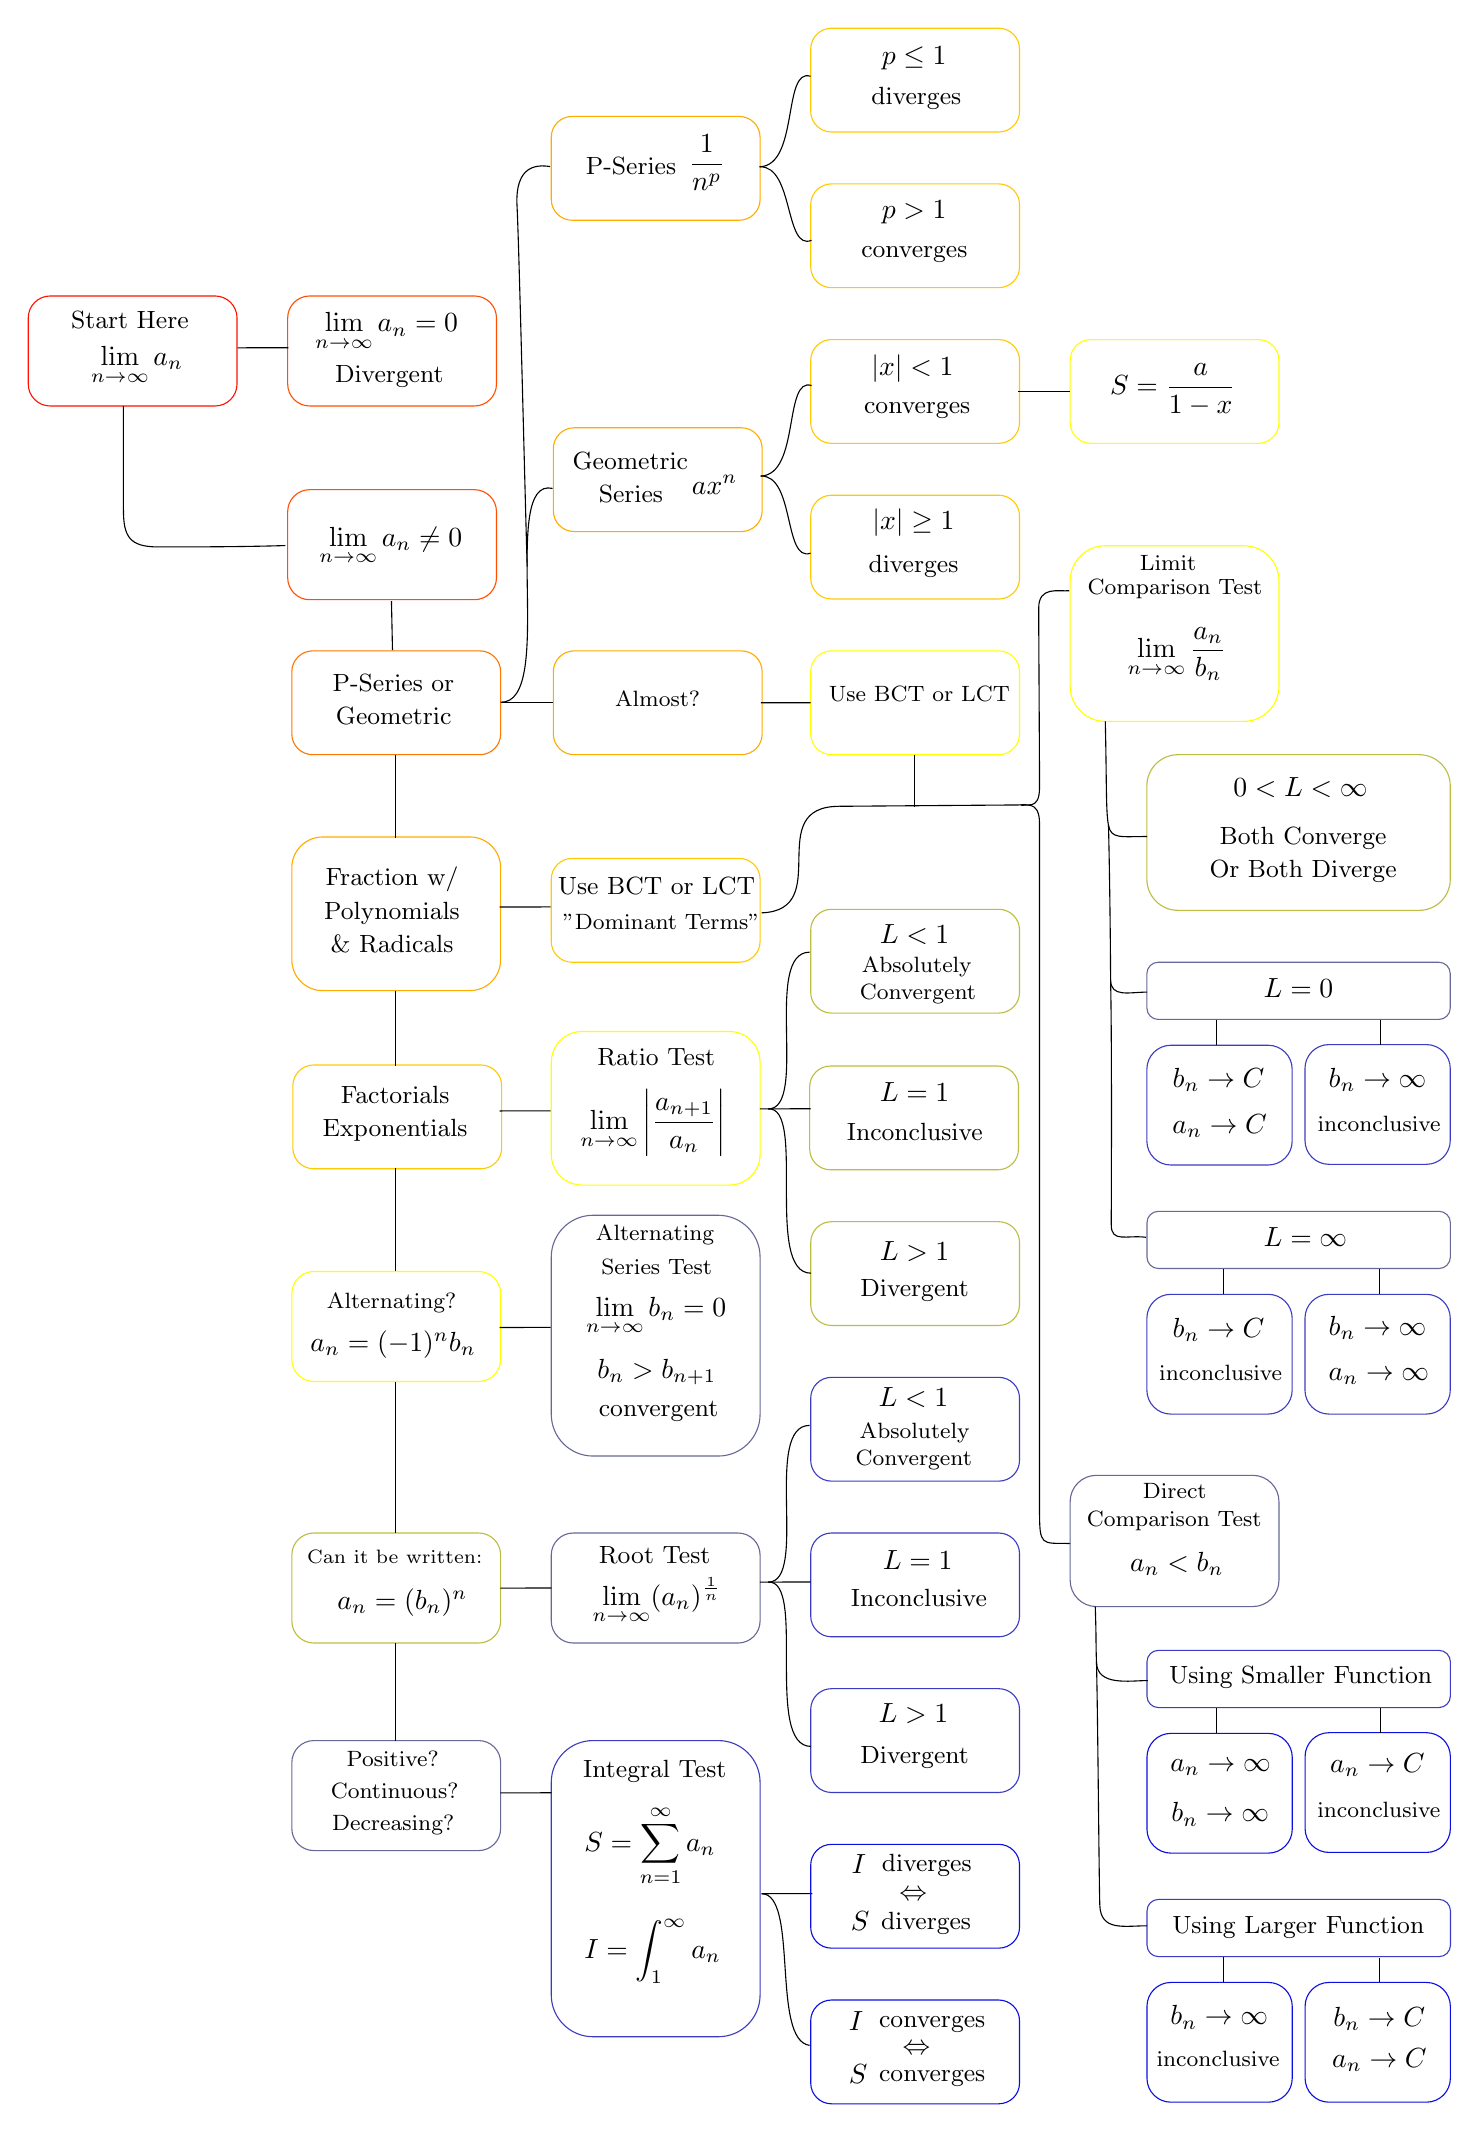
\begin{tikzpicture}[x=0.75pt,y=0.75pt,yscale=-1,xscale=1]
	
		%Lines
		%BEGIN_FOLD
		%Rounded Rect [id:dp5276780561916146] 
		\draw[red1]   (123,139.6) .. controls (123,133.75) and (127.75,129) .. (133.6,129) -- (213,129) .. controls (218.85,129) and (223.6,133.75) .. (223.6,139.6) -- (223.6,171.4) .. controls (223.6,177.25) and (218.85,182) .. (213,182) -- (133.6,182) .. controls (127.75,182) and (123,177.25) .. (123,171.4) -- cycle ;
		%Rounded Rect [id:dp23217052933469273] 
		\draw[red3]   (250,310) .. controls (250,304.48) and (254.48,300) .. (260,300) -- (340.6,300) .. controls (346.12,300) and (350.6,304.48) .. (350.6,310) -- (350.6,340) .. controls (350.6,345.52) and (346.12,350) .. (340.6,350) -- (260,350) .. controls (254.48,350) and (250,345.52) .. (250,340) -- cycle ;
		%Rounded Rect [id:dp7917994846918226] 
		\draw[red4]   (250,404.46) .. controls (250,396.29) and (256.63,389.66) .. (264.8,389.66) -- (335.8,389.66) .. controls (343.97,389.66) and (350.6,396.29) .. (350.6,404.46) -- (350.6,448.86) .. controls (350.6,457.04) and (343.97,463.66) .. (335.8,463.66) -- (264.8,463.66) .. controls (256.63,463.66) and (250,457.04) .. (250,448.86) -- cycle ;
		%Rounded Rect [id:dp6954021703001823] 
		\draw[red5]   (250.5,509.5) .. controls (250.5,503.98) and (254.98,499.5) .. (260.5,499.5) -- (341.1,499.5) .. controls (346.62,499.5) and (351.1,503.98) .. (351.1,509.5) -- (351.1,539.5) .. controls (351.1,545.02) and (346.62,549.5) .. (341.1,549.5) -- (260.5,549.5) .. controls (254.98,549.5) and (250.5,545.02) .. (250.5,539.5) -- cycle ;
		%Rounded Rect [id:dp9535410503024166] 
		\draw[red6]   (250,609.6) .. controls (250,603.75) and (254.75,599) .. (260.6,599) -- (340,599) .. controls (345.85,599) and (350.6,603.75) .. (350.6,609.6) -- (350.6,641.4) .. controls (350.6,647.25) and (345.85,652) .. (340,652) -- (260.6,652) .. controls (254.75,652) and (250,647.25) .. (250,641.4) -- cycle ;
		%Rounded Rect [id:dp5562441324605811] 
		\draw[red7]   (250,735.6) .. controls (250,729.75) and (254.75,725) .. (260.6,725) -- (340,725) .. controls (345.85,725) and (350.6,729.75) .. (350.6,735.6) -- (350.6,767.4) .. controls (350.6,773.25) and (345.85,778) .. (340,778) -- (260.6,778) .. controls (254.75,778) and (250,773.25) .. (250,767.4) -- cycle ;
		%Rounded Rect [id:dp002612931917562733] 
		\draw[red9]   (250,835.6) .. controls (250,829.75) and (254.75,825) .. (260.6,825) -- (340,825) .. controls (345.85,825) and (350.6,829.75) .. (350.6,835.6) -- (350.6,867.4) .. controls (350.6,873.25) and (345.85,878) .. (340,878) -- (260.6,878) .. controls (254.75,878) and (250,873.25) .. (250,867.4) -- cycle ;
		%Rounded Rect [id:dp976841386569514] 
		\draw[red2]   (248,232.93) .. controls (248,227.08) and (252.75,222.33) .. (258.6,222.33) -- (338,222.33) .. controls (343.85,222.33) and (348.6,227.08) .. (348.6,232.93) -- (348.6,264.73) .. controls (348.6,270.59) and (343.85,275.33) .. (338,275.33) -- (258.6,275.33) .. controls (252.75,275.33) and (248,270.59) .. (248,264.73) -- cycle ;
		%Rounded Rect [id:dp05785075235983772] 
		\draw[red4]   (376,202.5) .. controls (376,196.98) and (380.48,192.5) .. (386,192.5) -- (466.6,192.5) .. controls (472.12,192.5) and (476.6,196.98) .. (476.6,202.5) -- (476.6,232.5) .. controls (476.6,238.02) and (472.12,242.5) .. (466.6,242.5) -- (386,242.5) .. controls (380.48,242.5) and (376,238.02) .. (376,232.5) -- cycle ;
		%Rounded Rect [id:dp30887298474385627] 
		\draw[red4]   (376,310) .. controls (376,304.48) and (380.48,300) .. (386,300) -- (466.6,300) .. controls (472.12,300) and (476.6,304.48) .. (476.6,310) -- (476.6,340) .. controls (476.6,345.52) and (472.12,350) .. (466.6,350) -- (386,350) .. controls (380.48,350) and (376,345.52) .. (376,340) -- cycle ;
		%Straight Lines [id:da3348889158539843] 
		\draw    (375.6,324.71) -- (350.6,324.71) ;
		%Curve Lines [id:da11127512321326383] 
		\draw    (350.6,324.71) .. controls (377.6,325.71) and (349.6,215.71) .. (375.6,221.71) ;
		%Rounded Rect [id:dp6182832934916931] 
		\draw[red4]  (375,52.5) .. controls (375,46.98) and (379.48,42.5) .. (385,42.5) -- (465.6,42.5) .. controls (471.12,42.5) and (475.6,46.98) .. (475.6,52.5) -- (475.6,82.5) .. controls (475.6,88.02) and (471.12,92.5) .. (465.6,92.5) -- (385,92.5) .. controls (379.48,92.5) and (375,88.02) .. (375,82.5) -- cycle ;
		%Rounded Rect [id:dp8119892541022702] 
		\draw[red5]   (500,10) .. controls (500,4.48) and (504.48,0) .. (510,0) -- (590.6,0) .. controls (596.12,0) and (600.6,4.48) .. (600.6,10) -- (600.6,40) .. controls (600.6,45.52) and (596.12,50) .. (590.6,50) -- (510,50) .. controls (504.48,50) and (500,45.52) .. (500,40) -- cycle ;
		%Rounded Rect [id:dp7371895224055407] 
		\draw[red5]   (500,85) .. controls (500,79.48) and (504.48,75) .. (510,75) -- (590.6,75) .. controls (596.12,75) and (600.6,79.48) .. (600.6,85) -- (600.6,115) .. controls (600.6,120.52) and (596.12,125) .. (590.6,125) -- (510,125) .. controls (504.48,125) and (500,120.52) .. (500,115) -- cycle ;
		%Rounded Rect [id:dp7074739589926726] 
		\draw[red5]  (500,160) .. controls (500,154.48) and (504.48,150) .. (510,150) -- (590.6,150) .. controls (596.12,150) and (600.6,154.48) .. (600.6,160) -- (600.6,190) .. controls (600.6,195.52) and (596.12,200) .. (590.6,200) -- (510,200) .. controls (504.48,200) and (500,195.52) .. (500,190) -- cycle ;
		%Rounded Rect [id:dp6578888650262109] 
		\draw[red5]   (500,235) .. controls (500,229.48) and (504.48,225) .. (510,225) -- (590.6,225) .. controls (596.12,225) and (600.6,229.48) .. (600.6,235) -- (600.6,265) .. controls (600.6,270.52) and (596.12,275) .. (590.6,275) -- (510,275) .. controls (504.48,275) and (500,270.52) .. (500,265) -- cycle ;
		%Rounded Rect [id:dp28973955315794053] 
		\draw[red6]   (500,310) .. controls (500,304.48) and (504.48,300) .. (510,300) -- (590.6,300) .. controls (596.12,300) and (600.6,304.48) .. (600.6,310) -- (600.6,340) .. controls (600.6,345.52) and (596.12,350) .. (590.6,350) -- (510,350) .. controls (504.48,350) and (500,345.52) .. (500,340) -- cycle ;
		%Rounded Rect [id:dp4007938491245371] 
		\draw[red5]   (375,410) .. controls (375,404.48) and (379.48,400) .. (385,400) -- (465.6,400) .. controls (471.12,400) and (475.6,404.48) .. (475.6,410) -- (475.6,440) .. controls (475.6,445.52) and (471.12,450) .. (465.6,450) -- (385,450) .. controls (379.48,450) and (375,445.52) .. (375,440) -- cycle ;
		%Rounded Rect [id:dp37677039239315224] 
		\draw[red6]   (375,498.16) .. controls (375,489.99) and (381.63,483.36) .. (389.8,483.36) -- (460.8,483.36) .. controls (468.97,483.36) and (475.6,489.99) .. (475.6,498.16) -- (475.6,542.56) .. controls (475.6,550.74) and (468.97,557.36) .. (460.8,557.36) -- (389.8,557.36) .. controls (381.63,557.36) and (375,550.74) .. (375,542.56) -- cycle ;
		%Rounded Rect [id:dp1111312862120657] 
		\draw[red7]   (500,434.5) .. controls (500,428.98) and (504.48,424.5) .. (510,424.5) -- (590.6,424.5) .. controls (596.12,424.5) and (600.6,428.98) .. (600.6,434.5) -- (600.6,464.5) .. controls (600.6,470.02) and (596.12,474.5) .. (590.6,474.5) -- (510,474.5) .. controls (504.48,474.5) and (500,470.02) .. (500,464.5) -- cycle ;
		%Rounded Rect [id:dp2607251058181812] 
		\draw[red7]   (499.5,510) .. controls (499.5,504.48) and (503.98,500) .. (509.5,500) -- (590.1,500) .. controls (595.62,500) and (600.1,504.48) .. (600.1,510) -- (600.1,540) .. controls (600.1,545.52) and (595.62,550) .. (590.1,550) -- (509.5,550) .. controls (503.98,550) and (499.5,545.52) .. (499.5,540) -- cycle ;
		%Rounded Rect [id:dp43920416362763404] 
		\draw[red7]   (500,585) .. controls (500,579.48) and (504.48,575) .. (510,575) -- (590.6,575) .. controls (596.12,575) and (600.6,579.48) .. (600.6,585) -- (600.6,615) .. controls (600.6,620.52) and (596.12,625) .. (590.6,625) -- (510,625) .. controls (504.48,625) and (500,620.52) .. (500,615) -- cycle ;
		%Rounded Rect [id:dp40014483547563473] 
		\draw[red9]   (375,592.03) .. controls (375,580.92) and (384.01,571.91) .. (395.12,571.91) -- (455.48,571.91) .. controls (466.59,571.91) and (475.6,580.92) .. (475.6,592.03) -- (475.6,667.79) .. controls (475.6,678.9) and (466.59,687.91) .. (455.48,687.91) -- (395.12,687.91) .. controls (384.01,687.91) and (375,678.9) .. (375,667.79) -- cycle ;
		%Rounded Rect [id:dp44588110121134417] 
		\draw[red9]   (375,735.6) .. controls (375,729.75) and (379.75,725) .. (385.6,725) -- (465,725) .. controls (470.85,725) and (475.6,729.75) .. (475.6,735.6) -- (475.6,767.4) .. controls (475.6,773.25) and (470.85,778) .. (465,778) -- (385.6,778) .. controls (379.75,778) and (375,773.25) .. (375,767.4) -- cycle ;
		%Rounded Rect [id:dp5791282467060925] 
		\draw[red10]   (500,810) .. controls (500,804.48) and (504.48,800) .. (510,800) -- (590.6,800) .. controls (596.12,800) and (600.6,804.48) .. (600.6,810) -- (600.6,840) .. controls (600.6,845.52) and (596.12,850) .. (590.6,850) -- (510,850) .. controls (504.48,850) and (500,845.52) .. (500,840) -- cycle ;
		%Rounded Rect [id:dp007871882285400478] 
		\draw[red10]   (500,735) .. controls (500,729.48) and (504.48,725) .. (510,725) -- (590.6,725) .. controls (596.12,725) and (600.6,729.48) .. (600.6,735) -- (600.6,765) .. controls (600.6,770.52) and (596.12,775) .. (590.6,775) -- (510,775) .. controls (504.48,775) and (500,770.52) .. (500,765) -- cycle ;
		%Rounded Rect [id:dp6359084265783173] 
		\draw[red10]   (500,660) .. controls (500,654.48) and (504.48,650) .. (510,650) -- (590.6,650) .. controls (596.12,650) and (600.6,654.48) .. (600.6,660) -- (600.6,690) .. controls (600.6,695.52) and (596.12,700) .. (590.6,700) -- (510,700) .. controls (504.48,700) and (500,695.52) .. (500,690) -- cycle ;
		%Curve Lines [id:da48502447301873386] 
		\draw    (475.4,66.76) .. controls (494.4,66.16) and (486.4,18.66) .. (499.9,23.16) ;
		%Curve Lines [id:da032484372203260614] 
		\draw    (475.4,66.76) .. controls (491.9,66.16) and (487.4,107.66) .. (500.4,102.16) ;
		%Curve Lines [id:da195691268910809] 
		\draw    (363.4,259.36) .. controls (362.66,237.56) and (359.5,104.6) .. (358.5,85.6) .. controls (357.5,66.6) and (367.36,65.49) .. (374.4,66.66) ;
		%Curve Lines [id:da8831422898880397] 
		\draw    (475.9,215.76) .. controls (494.9,215.16) and (486.9,167.66) .. (500.4,172.16) ;
		%Curve Lines [id:da8233936863863811] 
		\draw    (475.9,215.76) .. controls (492.4,215.16) and (486.93,257.58) .. (499.93,252.91) ;
		%Rounded Rect [id:dp342008884816865] 
		\draw[red6]   (625,160) .. controls (625,154.48) and (629.48,150) .. (635,150) -- (715.6,150) .. controls (721.12,150) and (725.6,154.48) .. (725.6,160) -- (725.6,190) .. controls (725.6,195.52) and (721.12,200) .. (715.6,200) -- (635,200) .. controls (629.48,200) and (625,195.52) .. (625,190) -- cycle ;
		%Straight Lines [id:da7476248586368932] 
		\draw    (600,175) -- (625,175) ;
		%Straight Lines [id:da682118088194245] 
		\draw    (500,325) -- (476,324.96) ;
		%Curve Lines [id:da8330404360060142] 
		\draw    (479.5,520.66) .. controls (498.1,519.36) and (477.47,599.82) .. (500.13,599.82) ;
		%Curve Lines [id:da7842642400964113] 
		\draw    (479.5,520.66) .. controls (499.1,520.86) and (476.8,445.15) .. (499.47,445.15) ;
		%Straight Lines [id:da12262977175240541] 
		\draw    (475.5,520.65) -- (500,520.59) ;
		%Curve Lines [id:da2298417291600261] 
		\draw    (479.5,748.66) .. controls (498.1,747.36) and (477.47,827.82) .. (500.13,827.82) ;
		%Curve Lines [id:da8282341786918721] 
		\draw    (479.5,748.66) .. controls (499.1,748.86) and (476.8,673.15) .. (499.47,673.15) ;
		%Straight Lines [id:da752027771590952] 
		\draw    (475.5,748.65) -- (500,748.59) ;
		%Straight Lines [id:da19996319664097184] 
		\draw    (350.17,521.65) -- (374.67,521.59) ;
		%Straight Lines [id:da2860582855765246] 
		\draw    (350.17,423.41) -- (374.67,423.35) ;
		%Straight Lines [id:da5736905741390836] 
		\draw    (350.17,625.98) -- (356.53,625.97) -- (374.67,625.92) ;
		%Straight Lines [id:da26007296590851947] 
		\draw    (350.5,751.54) -- (356.87,751.53) -- (375,751.48) ;
		%Straight Lines [id:da026382565021525695] 
		\draw    (300,350) -- (300,390) ;
		%Straight Lines [id:da1000994781004183] 
		\draw    (300,464) -- (300,500) ;
		%Straight Lines [id:da13495592574538806] 
		\draw    (300,549) -- (300,599) ;
		%Straight Lines [id:da8867371344137516] 
		\draw    (300,652) -- (300,725) ;
		%Straight Lines [id:da28028117013293685] 
		\draw    (300,778) -- (300,825) ;
		%Rounded Rect [id:dp9338360889782491] 
		\draw[red10]   (375,845.12) .. controls (375,834.01) and (384.01,825) .. (395.12,825) -- (455.48,825) .. controls (466.59,825) and (475.6,834.01) .. (475.6,845.12) -- (475.6,947.57) .. controls (475.6,958.68) and (466.59,967.69) .. (455.48,967.69) -- (395.12,967.69) .. controls (384.01,967.69) and (375,958.68) .. (375,947.57) -- cycle ;
		%Curve Lines [id:da8854077421773605] 
		\draw    (476.33,898.78) .. controls (494.33,898.78) and (480.8,969.49) .. (499.47,971.84) ;
		%Straight Lines [id:da465766881319319] 
		\draw    (350.5,850.21) -- (356.87,850.19) -- (375,850.15) ;
		%Straight Lines [id:da9088072388317447] 
		\draw    (476.33,898.78) -- (500.83,898.72) ;
		%Curve Lines [id:da9679073340455149] 
		\draw    (476.3,426.21) .. controls (511.8,424.87) and (476.3,374.87) .. (513.8,374.87) ;
		%Straight Lines [id:da371181975966165] 
		\draw    (513.8,374.87) -- (601.2,374.21) ;
		%Straight Lines [id:da3590786403144586] 
		\draw    (550,350) -- (550,375) ;
		%Rounded Rect [id:dp4004105492466312] 
		\draw[red7]   (661.96,365) .. controls (661.96,356.72) and (668.67,350) .. (676.96,350) -- (793.13,350) .. controls (801.42,350) and (808.13,356.72) .. (808.13,365) -- (808.13,410) .. controls (808.13,418.28) and (801.42,425) .. (793.13,425) -- (676.96,425) .. controls (668.67,425) and (661.96,418.28) .. (661.96,410) -- cycle ;
		%Curve Lines [id:da6611306142125017] 
		\draw    (601.2,374.21) .. controls (603.46,373.27) and (610.24,377.48) .. (610.24,365.88) .. controls (610.24,354.28) and (609.84,290.2) .. (609.84,279.4) .. controls (609.84,268.6) and (619.44,271.48) .. (624.64,271) ;
		%Curve Lines [id:da7251917923941098] 
		\draw    (601.2,374.21) .. controls (602.41,375.16) and (610.24,371.08) .. (610.24,383.16) .. controls (610.24,395.24) and (610.24,695.64) .. (610.24,713.64) .. controls (610.24,731.64) and (610.88,729.81) .. (625.04,730.04) ;
		%Rounded Rect [id:dp9781901286558259] 
		\draw[red6]   (625,266.26) .. controls (625,256.91) and (632.58,249.33) .. (641.92,249.33) -- (708.67,249.33) .. controls (718.02,249.33) and (725.6,256.91) .. (725.6,266.26) -- (725.6,317.03) .. controls (725.6,326.38) and (718.02,333.96) .. (708.67,333.96) -- (641.92,333.96) .. controls (632.58,333.96) and (625,326.38) .. (625,317.03) -- cycle ;
		%Rounded Rect [id:dp28948379176832106] 
		\draw[red9]   (661.96,455.51) .. controls (661.96,452.47) and (664.43,450) .. (667.47,450) -- (802.62,450) .. controls (805.67,450) and (808.13,452.47) .. (808.13,455.51) -- (808.13,472.05) .. controls (808.13,475.09) and (805.67,477.56) .. (802.62,477.56) -- (667.47,477.56) .. controls (664.43,477.56) and (661.96,475.09) .. (661.96,472.05) -- cycle ;
		%Rounded Rect [id:dp4761251562543596] 
		\draw[red10]   (661.96,501.54) .. controls (661.96,495.17) and (667.12,490) .. (673.5,490) -- (720.42,490) .. controls (726.79,490) and (731.96,495.17) .. (731.96,501.54) -- (731.96,536.15) .. controls (731.96,542.53) and (726.79,547.69) .. (720.42,547.69) -- (673.5,547.69) .. controls (667.12,547.69) and (661.96,542.53) .. (661.96,536.15) -- cycle ;
		%Rounded Rect [id:dp16719764322274155] 
		\draw[red10]   (738.13,501.21) .. controls (738.13,494.83) and (743.3,489.67) .. (749.67,489.67) -- (796.59,489.67) .. controls (802.97,489.67) and (808.13,494.83) .. (808.13,501.21) -- (808.13,535.82) .. controls (808.13,542.19) and (802.97,547.36) .. (796.59,547.36) -- (749.67,547.36) .. controls (743.3,547.36) and (738.13,542.19) .. (738.13,535.82) -- cycle ;
		%Rounded Rect [id:dp007506369554147518] 
		\draw[red9]   (662,575.51) .. controls (662,572.47) and (664.47,570) .. (667.51,570) -- (802.66,570) .. controls (805.71,570) and (808.18,572.47) .. (808.18,575.51) -- (808.18,592.05) .. controls (808.18,595.09) and (805.71,597.56) .. (802.66,597.56) -- (667.51,597.56) .. controls (664.47,597.56) and (662,595.09) .. (662,592.05) -- cycle ;
		%Rounded Rect [id:dp6506664514902745] 
		\draw[red10]   (661.96,621.54) .. controls (661.96,615.17) and (667.12,610) .. (673.5,610) -- (720.42,610) .. controls (726.79,610) and (731.96,615.17) .. (731.96,621.54) -- (731.96,656.15) .. controls (731.96,662.53) and (726.79,667.69) .. (720.42,667.69) -- (673.5,667.69) .. controls (667.12,667.69) and (661.96,662.53) .. (661.96,656.15) -- cycle ;
		%Rounded Rect [id:dp6007608397646189] 
		\draw[red10]   (738.13,621.54) .. controls (738.13,615.17) and (743.3,610) .. (749.67,610) -- (796.59,610) .. controls (802.97,610) and (808.13,615.17) .. (808.13,621.54) -- (808.13,656.15) .. controls (808.13,662.53) and (802.97,667.69) .. (796.59,667.69) -- (749.67,667.69) .. controls (743.3,667.69) and (738.13,662.53) .. (738.13,656.15) -- cycle ;
		%Curve Lines [id:da3988020152144309] 
		\draw    (641.92,333.96) .. controls (642.63,363.71) and (642.15,377.52) .. (643.47,384.09) .. controls (644.78,390.67) and (649.15,389.43) .. (662.13,389.43) ;
		%Curve Lines [id:da07524555446658798] 
		\draw    (643.47,384.09) .. controls (644.17,413.84) and (644.47,449.59) .. (644.47,458.39) .. controls (644.47,467.19) and (653.47,464.39) .. (662.13,464.39) ;
		%Curve Lines [id:da43366112065621976] 
		\draw    (644.47,458.39) .. controls (645.17,488.14) and (644.8,567.72) .. (644.8,576.52) .. controls (644.8,585.32) and (652.13,581.32) .. (661.47,582.52) ;
		%Straight Lines [id:da9572104598470095] 
		\draw    (695.33,478) -- (695.33,490) ;
		%Straight Lines [id:da7518665472025012] 
		\draw    (774.33,477.67) -- (774.33,489.67) ;
		%Straight Lines [id:da6813080522559318] 
		\draw    (774,598) -- (774,610) ;
		%Straight Lines [id:da7973036316391295] 
		\draw    (698.67,597.67) -- (698.67,609.67) ;
		%Rounded Rect [id:dp842331742373688] 
		\draw[red9]   (625,709.85) .. controls (625,702.86) and (630.66,697.2) .. (637.65,697.2) -- (712.95,697.2) .. controls (719.94,697.2) and (725.6,702.86) .. (725.6,709.85) -- (725.6,747.79) .. controls (725.6,754.77) and (719.94,760.44) .. (712.95,760.44) -- (637.65,760.44) .. controls (630.66,760.44) and (625,754.77) .. (625,747.79) -- cycle ;
		%Rounded Rect [id:dp5659486550079835] 
		\draw[red10]   (662,787.04) .. controls (662,784) and (664.47,781.53) .. (667.51,781.53) -- (802.66,781.53) .. controls (805.71,781.53) and (808.18,784) .. (808.18,787.04) -- (808.18,803.58) .. controls (808.18,806.62) and (805.71,809.09) .. (802.66,809.09) -- (667.51,809.09) .. controls (664.47,809.09) and (662,806.62) .. (662,803.58) -- cycle ;
		%Rounded Rect [id:dp07710590767275671] 
		\draw[red11]   (662,833.07) .. controls (662,826.7) and (667.17,821.53) .. (673.54,821.53) -- (720.46,821.53) .. controls (726.83,821.53) and (732,826.7) .. (732,833.07) -- (732,867.68) .. controls (732,874.06) and (726.83,879.22) .. (720.46,879.22) -- (673.54,879.22) .. controls (667.17,879.22) and (662,874.06) .. (662,867.68) -- cycle ;
		%Rounded Rect [id:dp38528250250722906] 
		\draw[red11]   (738.18,832.74) .. controls (738.18,826.36) and (743.34,821.2) .. (749.71,821.2) -- (796.64,821.2) .. controls (803.01,821.2) and (808.18,826.36) .. (808.18,832.74) -- (808.18,867.35) .. controls (808.18,873.72) and (803.01,878.89) .. (796.64,878.89) -- (749.71,878.89) .. controls (743.34,878.89) and (738.18,873.72) .. (738.18,867.35) -- cycle ;
		%Rounded Rect [id:dp883885199216023] 
		\draw[red10]   (662.04,907.04) .. controls (662.04,904) and (664.51,901.53) .. (667.55,901.53) -- (802.71,901.53) .. controls (805.75,901.53) and (808.22,904) .. (808.22,907.04) -- (808.22,923.58) .. controls (808.22,926.62) and (805.75,929.09) .. (802.71,929.09) -- (667.55,929.09) .. controls (664.51,929.09) and (662.04,926.62) .. (662.04,923.58) -- cycle ;
		%Rounded Rect [id:dp503376311186928] 
		\draw[red11]   (662,953.07) .. controls (662,946.7) and (667.17,941.53) .. (673.54,941.53) -- (720.46,941.53) .. controls (726.83,941.53) and (732,946.7) .. (732,953.07) -- (732,987.68) .. controls (732,994.06) and (726.83,999.22) .. (720.46,999.22) -- (673.54,999.22) .. controls (667.17,999.22) and (662,994.06) .. (662,987.68) -- cycle ;
		%Rounded Rect [id:dp26874126789154795] 
		\draw[red11]   (738.18,953.07) .. controls (738.18,946.7) and (743.34,941.53) .. (749.71,941.53) -- (796.64,941.53) .. controls (803.01,941.53) and (808.18,946.7) .. (808.18,953.07) -- (808.18,987.68) .. controls (808.18,994.06) and (803.01,999.22) .. (796.64,999.22) -- (749.71,999.22) .. controls (743.34,999.22) and (738.18,994.06) .. (738.18,987.68) -- cycle ;
		%Curve Lines [id:da4107328267797645] 
		\draw    (637.09,760.44) .. controls (637.68,778.08) and (637.28,775.76) .. (637.68,787.36) .. controls (638.08,798.96) and (653.81,796.08) .. (662.48,796.08) ;
		%Curve Lines [id:da15936589480737906] 
		\draw    (637.68,787.36) .. controls (638.39,817.11) and (638.88,891.44) .. (639.28,904.24) .. controls (639.68,917.04) and (650.88,914.24) .. (662.08,914.24) ;
		%Straight Lines [id:da9784997383088185] 
		\draw    (695.38,809.53) -- (695.38,821.53) ;
		%Straight Lines [id:da2838750603234612] 
		\draw    (774.38,809.2) -- (774.38,821.2) ;
		%Straight Lines [id:da2942640751248773] 
		\draw    (774.04,929.53) -- (774.04,941.53) ;
		%Straight Lines [id:da4095207951881006] 
		\draw    (698.71,929.2) -- (698.71,941.2) ;
		%Rounded Rect [id:dp14686245494817274] 
		\draw[red11]   (500,885) .. controls (500,879.48) and (504.48,875) .. (510,875) -- (590.6,875) .. controls (596.12,875) and (600.6,879.48) .. (600.6,885) -- (600.6,915) .. controls (600.6,920.52) and (596.12,925) .. (590.6,925) -- (510,925) .. controls (504.48,925) and (500,920.52) .. (500,915) -- cycle ;
		%Rounded Rect [id:dp6718538545993173] 
		\draw[red11]   (500,960) .. controls (500,954.48) and (504.48,950) .. (510,950) -- (590.6,950) .. controls (596.12,950) and (600.6,954.48) .. (600.6,960) -- (600.6,990) .. controls (600.6,995.52) and (596.12,1000) .. (590.6,1000) -- (510,1000) .. controls (504.48,1000) and (500,995.52) .. (500,990) -- cycle ;
		%Rounded Rect [id:dp5867487508413325] 
		\draw[red2]   (248,139.6) .. controls (248,133.75) and (252.75,129) .. (258.6,129) -- (338,129) .. controls (343.85,129) and (348.6,133.75) .. (348.6,139.6) -- (348.6,171.4) .. controls (348.6,177.25) and (343.85,182) .. (338,182) -- (258.6,182) .. controls (252.75,182) and (248,177.25) .. (248,171.4) -- cycle ;
		%Straight Lines [id:da6769187559717462] 
		\draw    (223.83,153.98) -- (248.33,153.92) ;
		%Curve Lines [id:da2913602861699862] 
		\draw    (168.84,182.12) .. controls (168.84,205.81) and (168.87,219.24) .. (168.87,231.91) .. controls (168.87,244.57) and (171.53,249.91) .. (185.53,249.91) .. controls (199.53,249.91) and (226.2,249.91) .. (246.87,249.24) ;
		%Straight Lines [id:da5222347080687255] 
		\draw    (298,276) -- (298.5,299.6) ;
		%END_FOLD%
		
		%Start
		%BEGIN_FOLD
			\draw (138,135) node [anchor=north west][inner sep=0.75pt]   [align=left] {{ {\small Start Here}}};
			\draw (152,152) node [anchor=north west][inner sep=0.75pt]    {$\displaystyle \lim _{n\rightarrow \infty } a_{n}$};
			

		
				%Divergent
				%BEGIN_FOLD
			\draw (260,135.79) node [anchor=north west][inner sep=0.75pt]    {$\displaystyle \lim _{n\rightarrow \infty } a_{n} =0$};
			\draw (268,161) node [anchor=north west][inner sep=0.75pt]   [align=left]{\begin{minipage}[lt]{41.57pt}\setlength\topsep{0pt}\begin{center}{\small  Divergent}\end{center}\end{minipage}};
			%END_FOLD
				
				%Limit is not zero
				%BEGIN_FOLD
				\draw (262,239) node [anchor=north west][inner sep=0.75pt]    {$\displaystyle \lim _{n\rightarrow \infty } a_{n} \neq 0$};

					%Geometric Or P-Series
					%BEGIN_FOLD
			\draw (264,310) node [anchor=north west][inner sep=0.75pt]   [align=left] {{ {\small P-Series or }}\\{{\footnotesize }}};
			\draw (270,318) node [anchor=north west][inner sep=0.75pt]   [align=left] {{ {\footnotesize  }}\\{{\small Geometric}}};

				%P-Series
				%BEGIN_FOLD%
			\draw (440,50) node [anchor=north west][inner sep=0.75pt]    {$\displaystyle \frac{1}{n^{p}}$};
			\draw (386,61) node [anchor=north west][inner sep=0.75pt]   [align=left] {{ {\small P-Series}}};
			
			
				%Less then 1
				\draw (533,7.5) node [anchor=north west][inner sep=0.75pt]    {$p\leq 1$};
				\draw (528,27) node [anchor=north west][inner sep=0.75pt]   [align=left] {\small diverges};
				
				%Greater Then 1
				\draw (533,82) node [anchor=north west][inner 	 sep=0.75pt]    {$p >1$};
				\draw (519,104) node [anchor=north west][inner sep=0.75pt]   [align=left] {{\small { converges}}};
			%END_FOLD
		
				%Geometric Series
				%BEGIN_FOLD
			\draw (384,203) node [anchor=north west][inner sep=0.75pt]   		[align=left] {\begin{minipage}[lt]{42.2pt}\setlength\topsep{0pt}
			{ {\small Geometric }} \begin{center}{ {\small Series}}
			\end{center} \end{minipage}};
			\draw (441.5,214) node [anchor=north west][inner sep=0.75pt]    {$\displaystyle ax^{n}$};
				
				%Less then 1
				\draw (528,155.9) node [anchor=north west][inner sep=0.75pt]    {$| x| < 1$};
				\draw (520,179.11) node [anchor=north west][inner sep=0.75pt]   [align=left] {{ {\small converges}}};
					
					%Sum
					\draw (643,160.4) node [anchor=north west][inner sep=0.75pt]    {$\displaystyle S=\frac{a}{1-x}$};
				
				%Greater then 1
				\draw (528.5,230.4) node [anchor=north west][inner sep=0.75pt]    {$| x| \geq 1$};
				\draw (522.5,252.71) node [anchor=north west][inner sep=0.75pt]   [align=left] {{\small { diverges}}};
			%END_FOLD
				
				%Almost
				%BEGIN_FOLD
			\draw (400,318) node [anchor=north west][inner sep=0.75pt]   [align=left] {{ {\footnotesize Almost? }}};
			\draw (503,315.81) node [anchor=north west][inner sep=0.75pt]   [align=left] {{ {\footnotesize Use BCT or LCT }}};
			%END_FOLD
			%END_FOLD

					%Fractions Polynomails and Radicals
					%BEGIN_FOLD
			\draw (263.1,403) node [anchor=north west][inner sep=0.75pt]   [align=left] {\begin{minipage}[lt]{50.86pt}\setlength\topsep{0pt}
			\begin{center}{\small {Fraction w/}}\\{\small { Polynomials }}\\{\small { \& Radicals}}\end{center}\end{minipage}};
			
				%Use LCT or BCT
				\draw (372.5,408.01) node [anchor=north west][inner sep=0.75pt]   [align=left] {{ {\small Use BCT or LCT }}};
				\draw (375,425.51) node [anchor=north west][inner sep=0.75pt]   [align=left] {{ {\footnotesize  "Dominant Terms" }}};
			%END_FOLD
	
					% Factorials Expontentials
					%BEGIN_FOLD
		\draw (262.1,508.5) node [anchor=north west][inner sep=0.75pt]   [align=left] {\begin{minipage}[lt]{54.6pt}\setlength\topsep{0pt}
		\begin{center}{ {\small Factorials}}\\{ {\small Exponentials}}\end{center}\end{minipage}};
	
			%Ratio Test
			\draw (392.1,490.33) node [anchor=north west][inner sep=0.75pt]   [align=left] {\begin{minipage}[lt]{48.26pt}\setlength\topsep{0pt}
			\begin{center}{ {\small Ratio Test}}\end{center}\end{minipage}};
			\draw (387.7,510) node [anchor=north west][inner sep=0.75pt]    {$\displaystyle \lim _{n\rightarrow \infty }\left| \frac{a_{n+1}}{a_{n}}\right| $};
	
				%Absolutley Convergent
				\draw (522.6,446.5) node [anchor=north west][inner sep=0.75pt]   [align=left] {\begin{minipage}[lt]{40.81pt}\setlength\topsep{0pt}
				\begin{center}{\footnotesize {Absolutely}}\end{center}\end{minipage}};
				\draw (532,430.4) node [anchor=north west][inner sep=0.75pt]    {$L< 1$};
				\draw (521.7,459.51) node [anchor=north west][inner sep=0.75pt]   [align=left]{\begin{minipage}[lt]{43.05pt}\setlength\topsep{0pt}\begin{center}{\footnotesize { Convergent}}\end{center}\end{minipage}};
				
				%Inconclusive
				\draw (532,506.9) node [anchor=north west][inner sep=0.75pt]    {$L=1$};
				\draw (514.6,526.5) node [anchor=north west][inner sep=0.75pt]   [align=left]{\begin{minipage}[lt]{51.41pt}\setlength\topsep{0pt}\begin{center}{{\small Inconclusive}}\end{center}\end{minipage}};

				%Divergent
				\draw (532,583.4) node [anchor=north west][inner sep=0.75pt]    {$L >1$};
				\draw (521.1,601.5) node [anchor=north west][inner sep=0.75pt]   [align=left]{\begin{minipage}[lt]{41.57pt}\setlength\topsep{0pt}\begin{center}{\small { Divergent}}\end{center}\end{minipage}};
			
			
		%END_FOLD
				
					%Alternating
					%BEGIN_FOLD
			\draw (265.1,608) node [anchor=north west][inner sep=0.75pt]   [align=left]{\begin{minipage}[lt]{47.58pt}\setlength\topsep{0pt}\begin{center}{ {\footnotesize Alternating?}}\end{center}\end{minipage}};
			\draw (257.7,626.11) node [anchor=north west][inner sep=0.75pt]    {$a_{n} =( -1)^{n} b_{n}$};
				
				% Alternating Series Test
				\draw (394.6,575.5) node [anchor=north west][inner sep=0.75pt]   [align=left]{\begin{minipage}[lt]{43.72pt}\setlength\topsep{0pt}\begin{center}{{\footnotesize Alternating}}\end{center}\end{minipage}};
				\draw (397.1,592) node [anchor=north west][inner sep=0.75pt]   [align=left]{\begin{minipage}[lt]{41.1pt}\setlength\topsep{0pt}\begin{center}{{\footnotesize Series Test}}\end{center}\end{minipage}};
				\draw (390.5,610) node [anchor=north west][inner sep=0.75pt]    {$\displaystyle \lim _{n\rightarrow \infty } b_{n} =0$};
				\draw (396,640) node [anchor=north west][inner sep=0.75pt]    {$b_{n}  >b_{n+1}$};
				\draw (395.1,660) node [anchor=north west][inner sep=0.75pt]   [align=left]{\begin{minipage}[lt]{45.53pt}\setlength\topsep{0pt}\begin{center}{{\small convergent}}\end{center}\end{minipage}};
			%END_FOLD
	
					%Root Test
					%BEGIN_FOLD
			\draw (253,732) node [anchor=north west][inner sep=0.75pt]   [align=left]{\begin{minipage}[lt]{67.94pt}\setlength\topsep{0pt}\begin{center}{\scriptsize { Can it be written:}}\end{center}\end{minipage}};
			\draw (270.7,750.61) node [anchor=north west][inner sep=0.75pt]    {$a_{n} =( b_{n})^{n}$};
				
				%Root Test
				\draw (395.1,730) node [anchor=north west][inner sep=0.75pt]   [align=left]{\begin{minipage}[lt]{42.64pt}\setlength\topsep{0pt}\begin{center}{ {\small Root Test}}\end{center}\end{minipage}};
				\draw (393.7,745.11) node [anchor=north west][inner sep=0.75pt]    {$\displaystyle \lim _{n\rightarrow \infty }( a_{n})^{\frac{1}{n}}$};
					
					%Asolutley convergent
					\draw (531.5,653.68) node [anchor=north west][inner sep=0.75pt] {$L< 1$};
					\draw (521.6,670.78) node [anchor=north west][inner sep=0.75pt]   [align=left]{\begin{minipage}[lt]{40.81pt}\setlength\topsep{0pt}\begin{center}{\footnotesize {Absolutely}}\end{center}\end{minipage}};
					\draw (519.7,683.8) node [anchor=north west][inner sep=0.75pt]   [align=left]{\begin{minipage}[lt]{43.05pt}\setlength\topsep{0pt}\begin{center}{\footnotesize {Convergent}}\end{center}\end{minipage}};
					
					%Inconclusive
					\draw (533.5,732.18) node [anchor=north west][inner sep=0.75pt]{$L=1$};
					\draw (516.6,750.78) node [anchor=north west][inner sep=0.75pt]   [align=left]{\begin{minipage}[lt]{51.41pt}\setlength\topsep{0pt}\begin{center}{{\small Inconclusive}}\end{center}\end{minipage}};
					
					%Divergent
					\draw (531.5,806.) node [anchor=north west][inner sep=0.75pt]{$L >1$};
					\draw (521.1,826.78) node [anchor=north west][inner sep=0.75pt]   [align=left]{\begin{minipage}[lt]{41.57pt}\setlength\topsep{0pt}\begin{center}{\small { Divergent}}\end{center}\end{minipage}};
	
			%END_FOLD
		
					%Integral Test
					%BEGIN_FOLD
		\draw (274.27,829.) node [anchor=north west][inner sep=0.75pt]   [align=left]{\begin{minipage}[lt]{34.57pt}\setlength\topsep{0pt}\begin{center}{{\footnotesize Positive?}}\end{center}\end{minipage}};
		\draw (267.53,835.55) node [anchor=north west][inner sep=0.75pt]   [align=left]{\begin{minipage}[lt]{42.63pt}\setlength\topsep{0pt}\begin{center}{{\footnotesize Continuous?}}\end{center}\end{minipage}};
		\draw (267.53,859.88) node [anchor=north west][inner sep=0.75pt]   [align=left]{\begin{minipage}[lt]{45.02pt}\setlength\topsep{0pt}\begin{center}{{\footnotesize Decreasing?}}\end{center}\end{minipage}};
			
			\draw (387.6,833) node [anchor=north west][inner sep=0.75pt]   [align=left]{\begin{minipage}[lt]{53.99pt}\setlength\topsep{0pt}\begin{center}{{\small Integral Test}}\end{center}\end{minipage}};
			\draw (383,854.94) node [anchor=north west][inner sep=0.75pt]{$ \begin{array}{l} {\displaystyle S=\sum _{n=1}^{\infty } a_{n}}\\ \\ {\displaystyle I=\int\nolimits _{1}^{\infty } a_{n}} \end{array}$};
				
				\draw (518.4,878.75) node [anchor=north west][inner sep=0.75pt] {$I$};
				\draw (531.43,878.69) node [anchor=north west][inner sep=0.75pt]   [align=left]{\begin{minipage}[lt]{34.88pt}\setlength\topsep{0pt}\begin{center}{{\small diverges}}\end{center}\end{minipage}};
				
				\draw (518.07,906.09) node [anchor=north west][inner sep=0.75pt] {$S$};
				\draw (531.1,906.35) node [anchor=north west][inner sep=0.75pt]   [align=left]{\begin{minipage}[lt]{34.88pt}\setlength\topsep{0pt}\begin{center}{{\small diverges}}\end{center}\end{minipage}};
				
				\draw (541.5,896.09) node [anchor=north west][inner sep=0.75pt]    {$\Leftrightarrow$};
				
				\draw (517.07,954.42) node [anchor=north west][inner sep=0.75pt]    {$I$};
				\draw (530.1,957.02) node [anchor=north west][inner sep=0.75pt]   [align=left]{\begin{minipage}[lt]{40.75pt}\setlength\topsep{0pt}\begin{center}{\small converges}\end{center}\end{minipage}};
				\draw (543,970) node [anchor=north west][inner sep=0.75pt]    {$\Leftrightarrow $};
				\draw (517.07,980) node [anchor=north west][inner sep=0.75pt]{$S$};
				\draw (530.1,983) node [anchor=north west][inner sep=0.75pt]   [align=left]{\begin{minipage}[lt]{40.75pt}\setlength\topsep{0pt}\begin{center}{\small converges}\end{center}\end{minipage}};
		%END_FOLD

					%Limit Comparison Test
					%BEGIN_FOLD
		\draw (657.33,252.81) node [anchor=north west][inner sep=0.75pt]   [align=left] {{\footnotesize {Limit}}};
		\draw (632.13,264.29) node [anchor=north west][inner sep=0.75pt]   [align=left] {{\footnotesize {Comparison Test}}};
		\draw (651.37,287.28) node [anchor=north west][inner sep=0.75pt]    {$\displaystyle \lim _{n\rightarrow \infty }\frac{a_{n}}{b_{n}}$};

			%Between Zero and Infty
			\draw (702.37,359.95) node [anchor=north west][inner sep=0.75pt]{$0< L< \infty $};
			\draw (689.47,383.63) node [anchor=north west][inner sep=0.75pt]   [align=left]{\begin{minipage}[lt]{69.74pt}\setlength\topsep{0pt}\begin{center}{{\small Both Converge}}\\{ {\small Or Both Diverge}}\end{center}\end{minipage}};
			
			
			%L=0
			\draw (717,456.61) node [anchor=north west][inner sep=0.75pt] {$L=0$};
				
				\draw (673.16,499.73) node [anchor=north west][inner sep=0.75pt]    {$b_{n}\rightarrow C$};
				\draw (673.,522.07) node [anchor=north west][inner sep=0.75pt]    {$a_{n}\rightarrow C$};
		
				\draw (748.29,499.94) node [anchor=north west][inner sep=0.75pt]    {$b_{n}\rightarrow \infty $};
				\draw (738.5,523) node [anchor=north west][inner sep=0.75pt]   [align=left] {{ {\footnotesize inconclusive}}};
		
			%L=inf
			\draw (717,576.61) node [anchor=north west][inner sep=0.75pt]    {$L=\infty $};
				
				\draw (748.29,619.09) node [anchor=north west][inner sep=0.75pt]    {$b_{n}\rightarrow \infty $};
				\draw (748.29,644.42) node [anchor=north west][inner sep=0.75pt]    {$a_{n}\rightarrow \infty $};

				\draw (673.16,620.09) node [anchor=north west][inner sep=0.75pt]    {$b_{n}\rightarrow C$};
				\draw (662.2,642.89) node [anchor=north west][inner sep=0.75pt]   [align=left] {{ {\footnotesize inconclusive}}};

		%END_FOLD
	
					%Direct Comparison Test
					%BEGIN_FOLD
		\draw (655,700) node [anchor=north west][inner sep=0.75pt]   [align=left] {{\footnotesize { Direct}}};
		\draw (628,713.2) node [anchor=north west][inner sep=0.75pt]   [align=left] {{\footnotesize { Comparison Test}}};
		\draw (652.6,733.) node [anchor=north west][inner sep=0.75pt]    	{$a_{n} < b_{n}$};
			
			\draw (667,788) node [anchor=north west][inner sep=0.75pt]   [align=left] {{ {\small Using Smaller Function}}};
				
				\draw (672,833) node [anchor=north west][inner sep=0.75pt]    {$a_{n}\rightarrow \infty $};
				\draw (672.5,853.65) node [anchor=north west][inner sep=0.75pt]    {$b_{n}\rightarrow \infty $};
				
				\draw (749,830) node [anchor=north west][inner sep=0.75pt]    {$a_{n}\rightarrow C$};
				\draw (738.4,853.57) node [anchor=north west][inner sep=0.75pt]   [align=left] {{ {\footnotesize inconclusive}}};
			
			
			\draw (668.5,908.6) node [anchor=north west][inner sep=0.75pt]   [align=left] {{ {\small Using Larger Function}}};
				\draw (750,972) node [anchor=north west][inner sep=0.75pt]    	{$a_{n}\rightarrow C$};
				\draw (750.5,952.) node [anchor=north west][inner sep=0.75pt]   {$b_{n}\rightarrow C$};
				
				\draw (672,951.5) node [anchor=north west][inner sep=0.75pt]    {$b_{n}\rightarrow \infty $};
				\draw (665.4,973.5) node [anchor=north west][inner sep=0.75pt]   [align=left] {\footnotesize inconclusive};
			%END_FOLD
			
				%END_FOLD
			
			%END_FOLD



	\end{tikzpicture}
	
	
	
	
	
	
	
	
	
	
	
	
	
\end{document}